\documentclass[titlepage]{article}
\usepackage{array}
\usepackage{enumerate}
\usepackage{graphicx}
\usepackage{listings}

\begin{document}

\author{Stevan Stanisic and Santana Mach}
\title{COMP 8505 - Final Project \\ Rootkit \\ Design Documents}
\date{Nov 06, 2011}
\maketitle{}

\tableofcontents
\pagebreak

\section{Introduction}

We are building our program from the foundation created by our previous covert channel and rootkit assignments. While we have explored the idea of creating a Passive Covert
Channel, we decided against it both because it would be more difficult to test and requires a compromised gateway router which must then forward the traffic to a known location.

The primary functionality that is being added for this project is the exfiltration function, the command function will be ported from existing code. As far as the covert channels go, we will again be primarily using existing code, although we would like to try an application layer covert channel as well as an ICMP based one to see if they are any easier or more difficult to detect.

As we would like this program to be suitable for use over the public internet, we will be introducing a simple reliability layer to allow for retransmission of corrupted or incomplete data.
Finally, we want to address a few issues with the existing code that we will be porting that might cause it to give itself away (eg. printing error messages to the screen). If time permits,
it would be nice to look installing the backdoor as a kernel module, however, that looks unlikely at the moment.

\section{Program Functionality}

The program will be made up of two executables, a Command and Control Client application and a Backdoor Server application.

The Client should have two modes, of which one will be active at a time:
\begin{itemize}
  \item Command Mode - In which the user can send commands to the Server and optionally receive responses.
  \item Exfiltration Mode - In which the user can update the watch list on the Server.
\end{itemize}

In both modes, the Client will also be listening for Exfiltration transmissions from the server and saving them to disk.

The Server will simultaneously be monitoring its network interfaces for incoming commands from the Client and its list of
watch directories for file changes.

The program will offer 3 different covert channel modes:
\begin{enumerate}
  \item UDP Header - Source Port
  \item NTP Payload - Root Dispersion
  \item ICMP Echo - Sequence Number
\end{enumerate}

The goal that we will be trying to attain is communication with a minimal footprint by which someone could identify and compromise our channel, to
that end we will be concentrating on secrecy and not raw throughput.

All of our communication will be encrypted using DES with a key that is stored in the configuration file.  Further, transmissions will be prefixed with a password,
however, if someone has broken our encryption, it is only a matter of time before they reverse engineer the protocol, so the value of the password is limited.
At best, we are buying ourselves a little bit more time.

\begin{lstlisting}
Pseudo-code for Client Program
{
  Main Function
  {
    Parse arguments;
    Read config file;

    Pass address into backdoor_client();
  }

  backdoor_client Function
  {
    Verify address and port;

    Setup listening_thread();

    While read stdin
    {
      if exfil switch is set
        set exfil path to send;

      Prepare raw socket;
    }
  }

  listen_thread Function
  {
    Prepare listening socket;

    While socket is open
    {
      Receive packet;
      Decrypt payload;
      Print decrypted payload;
    }
  }
}
\end{lstlisting}

\clearpage

\begin{lstlisting}
Pseudo-code for Server Program
{
  Main Function
  {
    Parse arguments;
    Read config file;

    Mask the process name;

    Pass filter into pcap_init();

    Execute srv_listen();
  }

  pcap_init Function
  {
    Open pcap packet capture;
    Build packet filter;
    Set packet filer;
  }

  srv_listen Function
  {
    Forever Loop
    {
      Process packet and pass into pkt_handler;
    }
  }

  pkt_handler Function
  {
    Locate payload portion of packet;

    Authenticate backdoor header key;

    Return if authentication fails;

    Decrypt payload with DES;

    Verify decrypted contents;

    Extract command from contents;

    Grab return address;

    Pass command and address into execute();
  }

  execute Function
  {
    Run command and grab standard out;

    Prepare raw socket for duplex;

    While content in stdout
    {
      Switch with covert mode;
      Encrypt content with DES;
      Send encrypted content to client;
    }   
  }

  covert_udplen Function
  {
    
  }

  covert_ntp Function
  {
    
  }

  covert_icmp Function
  {
    
  }

  exfil Function
  {

  }
}
\end{lstlisting}

\clearpage

\section{Communication Details}

As stated earlier, our goal is to be undetectable. To that end, all transmissions will be sent using raw sockets and all reception will be done using the pcap library; this will allow us to bypass
any local firewalls. If a suspicious admin was to send random probes to our Client machine, ideally it should not respond at all.  Whenever we are sending data we will do so slowly so that
there aren't any CPU usage or bandwidth spikes to draw attention to our covert channel.  The other advantage of transmitting more slowly it is less likely that our packets will be
reordered or dropped as we are adding minimal traffic to the channel, the only time a packet would be dropped would be on an already saturated channel. 

This will allow us to use a simpler reliability mechanism. As we want to minimize the amount of two way communication required by our covert channel, we will simply transmit some
redundancy data with the initial frame that will allow us to verify and acknowledge successful transmissions.  Bad hash values will signal corrupted data and timeouts will
signal dropped packets; both of these conditions will trigger a full retransmission.

\clearpage

\subsection{State Machine}

The client and the server will each possess a pair of threads to run each of their State Machines.  The basic interaction of each can be seen in the following diagram:

\begin{figure}[htb]                                                                       
  \begin{center}
    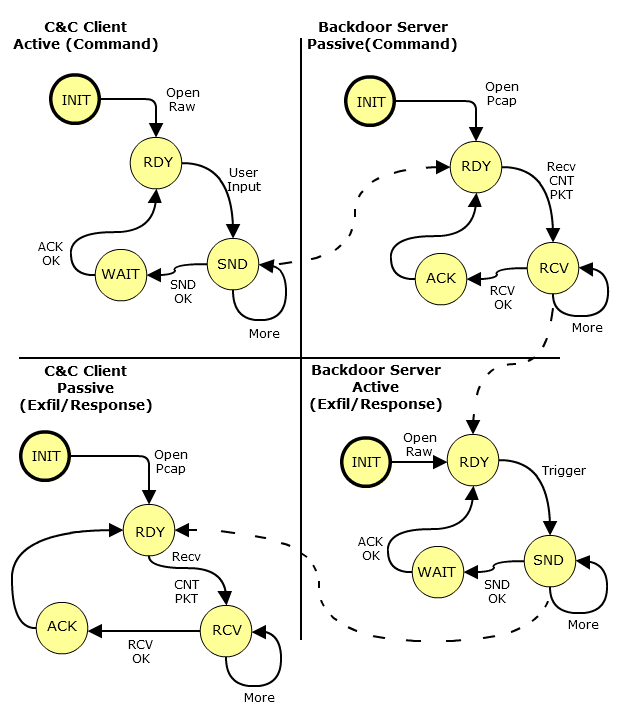
\includegraphics[width=0.9\textwidth]{imgs/std.png}
  \end{center}
  \caption{Program State Transition Diagram}
  \label{fig:std}
\end{figure}

Starting with the Client, it is the Active part in the Command role. It will ready itself and then send user input to the Server via the covert channel. The Server will then process
the command and optionally push the response to the Exfil/Response component to send back to the Client. In the Exfil/Response role, the Server is the Active party as it
initiates communication with the Client.

\clearpage

However, this does not cover the lower level operation as we are not using a reliable protocol like TCP, thus, we need to introduce a more detailed set of steps where the SND and RCV
bubbles in the previous diagram are.

\begin{figure}[htb]                                                                       
  \begin{center}
    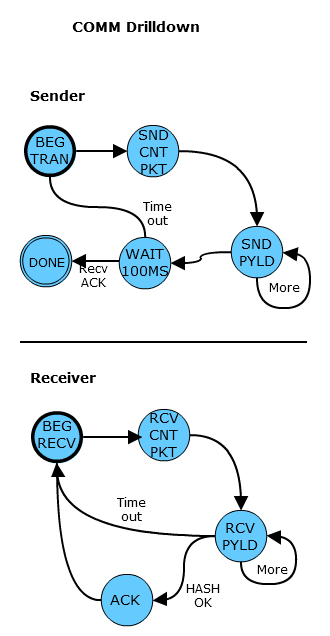
\includegraphics[width=0.5\textwidth]{imgs/comm.png}
  \end{center}
  \caption{Transmission State Transition Diagram}
  \label{fig:comm}
\end{figure}

These sub-states break down the expected behaviour when we are sending or receiving an individual transmission and cover the timeout and retransmission requirements we set
forth for our covert channel. The Control frame (CNT PKT) is discussed further in the Covert Channel section of the design.

\begin{lstlisting}
Pseudo-code for State Machine
{
  Send Machine
  {
    Prepare raw socket;
    
    Wait for command to trigger;
    
    While more to send
    {
      Send packet to receiving machine;
       
      Sleep to slow data stream;
    }
  }
  
  Receive Machine
  {
    Open pcap packet reading;
    
    Wait for trigger
    {
      Process packet;
      
      If last packet
      {
        If hash is incorrect
          Ask for retransmission;
        
        If server
          Send response or file;
      
        If client
          Display to command line;
      }
    }
  }
}
\end{lstlisting}

\clearpage

\subsection{Covert Channel}

In order to simplify covert channel handling, we will use the same internal format regardless of which program mode is selected. We will use 2 bytes for our covert channel
in whichever protocol we are using as a host. The format of the data we will be putting in those 2 bytes can be seen in the following diagram.

\begin{figure}[htb]                                                                       
  \begin{center}
    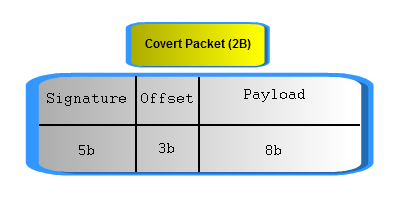
\includegraphics[width=0.9\textwidth]{imgs/packet.png}
  \end{center}
  \caption{Packet Data Diagram}
  \label{fig:packet}
\end{figure}

The 5 signature bits should be enough to uniquely identify our covert channel, although these should be different for each mode so that there isn't a single signature that can
be used to detect it. The 3 bit offset may not strictly be necessary as we will be sending slowly, but it would be unfortunate to lose data because our packets were reordered in
transit.  

Finally, we will only be sending 1 byte of data per packet, however, that causes an issue as we would like to be able to encrypt 64bits of data at a time. To that end
we will be building 8 byte frames. This means we need the ability to identify the length of a transmission as not all of them will fall on even 8 byte boundaries.  To solve this problem
(and a few others) we will introduce a Control frame.

\clearpage

\begin{figure}[htb]                                                                       
  \begin{center}
    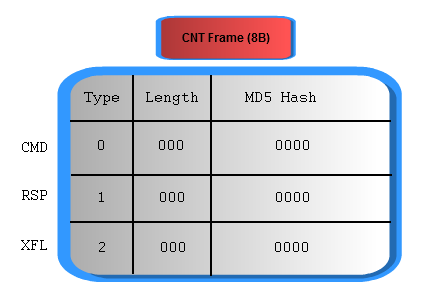
\includegraphics[width=0.9\textwidth]{imgs/frame.png}
  \end{center}
  \caption{Control Frame Diagram}
  \label{fig:frame}
\end{figure}

Inside the Control frame we are incuding a type field so that we can determine what type of request/response we are receiving, a length field so that we know in advance how
many bytes we can expect to receive, and a hash so that we can determine the validity of the data that we have received. In the interest of keeping our Control frame compact,
we will be using only 3 bytes for the length field, limiting us to 16MB transmissions; we believe that transmissions larger than that would be difficult to consider covert. 

Another shortcoming due to the small CNT frame size is that we are only using 4B of the MD5 hash, which means our chance of a hash collision is 1 in $2^{16}$, rather than the $2^{32}$
for the full hash value (note $n/2$ due to the birthday paradox). We feel that this is an acceptable tradeoff given the design goals we set earlier.

The overall structure of a transmission at a high level can be visualized as follows:

\clearpage

\begin{figure}[htb]                                                                       
  \begin{center}
    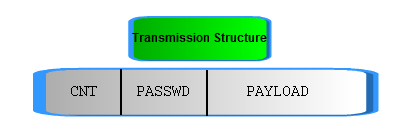
\includegraphics[width=0.9\textwidth]{imgs/transmission.png}
  \end{center}
  \caption{Overall Transmission Diagram}
  \label{fig:transmission}
\end{figure}

We will lead with the 8 byte control packet, followed by the pre-determined password and then the payload. The hash value will be calculated over the password and payload
portions of the transmission.

\clearpage

\section{Task Breakdown}

\begin{itemize}
	\item Extract old code [Santana]
	\item Reliability
	\subitem Retransmissions [Steve]
	\subitem Control Packets [Steve]
	\subitem Timeouts [Steve]
	\item Covert Raw Socket Crafting
	\subitem UDP Length Mode [Santana]
	\subitem NTP Mode [Santana]
	\subitem ICMP Mode [Santana]
	\item Exfiltration
	\subitem Client [Steve]
	\subitem Server [Santana]
\end{itemize}

\begin{figure}[htb]                                                                       
  \begin{center}
    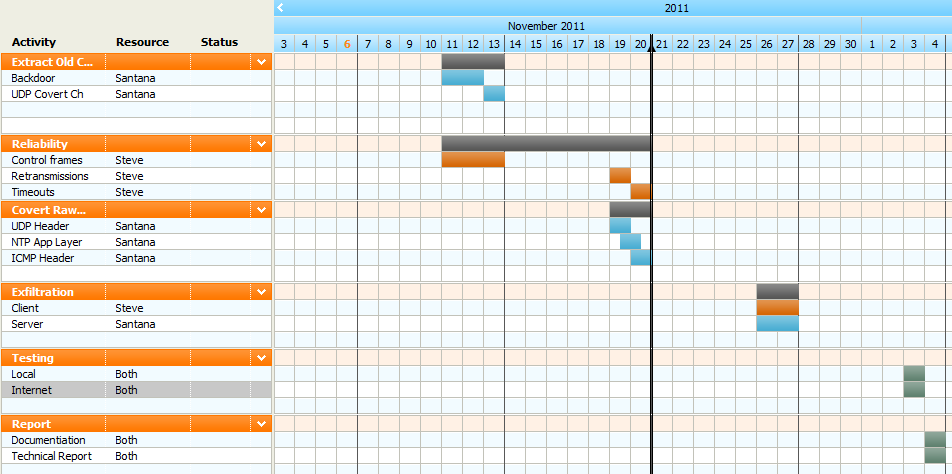
\includegraphics[width=0.5\textwidth]{imgs/timeline.png}
  \end{center}
  \caption{Project Timeline}
  \label{fig:timeline}
\end{figure}

We feel that the timeline is extremely tight in the testing and reporting phases, so we will attempt to begin these activities early, while development work is being done on the various
program components.

The only times we can firmly schedule for the project are on weekends, but if we see the schedule slipping, we have the option to add weekday hours as required to bring it back on
track.

\end{document}
